\documentclass{article}
\usepackage[utf8]{inputenc}

\title{Laboratorio03_INTELIGENCIA_NEGOCIOS}
\author{edwartbalcon}
\date{Septiembre 2021}

\usepackage[utf8]{inputenc}
\usepackage[spanish]{babel}
\usepackage{natbib}
\usepackage{graphicx}

\begin{document}

\title{Caratula}

\begin{titlepage}
\begin{center}
\begin{Large}
\textbf{UNIVERSIDAD PRIVADA DE TACNA} \\
\end{Large}
\vspace*{-0.025in}
\begin{figure}[htb]
\begin{center}

\includegraphics[width=6cm]{./images/logo_UPT}
\end{center}
\end{figure}
\vspace*{-0.025in}
\begin{Large}
\textbf{FACULTAD DE INGENIERIA} \\
\end{Large}
\vspace*{0.05in}
\begin{Large}
\textbf{Escuela Profesional de Ingeniería de Sistema} \\
\end{Large}


\vspace*{0.4in}

\vspace*{0.1in}
\begin{Large}
\textbf{Informe de laboratorio 09: Construyendo un ETL
Serverless} \\
\end{Large}

\vspace*{0.3in}
\begin{Large}
\textbf{Curso: Inteligencia de negocios} \\
\end{Large}

\vspace*{0.3in}
\begin{Large}
\textbf{DOCENTE: Ing. Patrick Cuadros Quiroga} \\
\end{Large}

\vspace*{0.2in}
\vspace*{0.1in}
\begin{large}

\begin{Large}
\textbf{Alumno: Balcon Coahila, Edwart Juan\hfill	(2013046516) } \\
\end{Large}

\vspace*{0.15in}
\begin{Large}
\textbf{Tacna – Perú} \\
\end{Large}

\vspace*{0.05in}
\begin{Large}
\textbf{2021 } \\
\end{Large}

\end{large}
\end{center}

\end{titlepage}


\newpage

\section{ Realizar los siguientes pasos para el laboratorio }

\textbf{1.1.  ) Entramos a la consola de AWS y accedemos al servicio de S3}

\begin{center}
		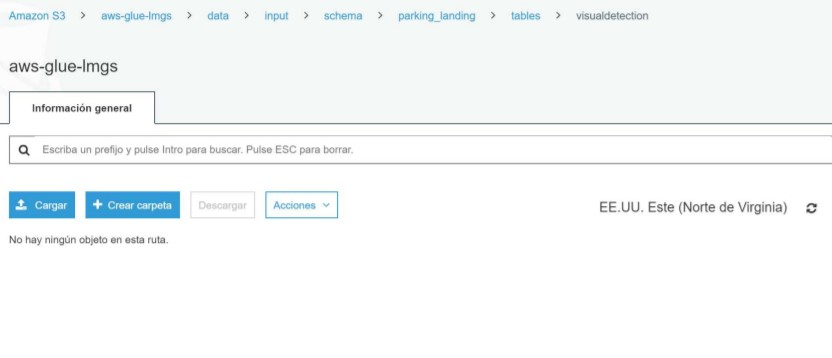
\includegraphics[width=15cm]{./images/1} 
	\end{center}
	
\textbf{1.2. Entrar al servicio de Glue}


    \begin{center}
		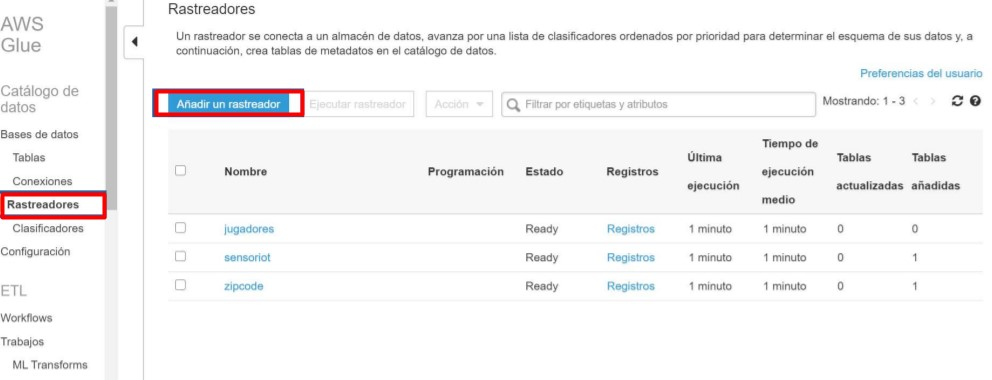
\includegraphics[width=15cm]{./images/2} 
	\end{center}

\textbf{1.3.   Agregamos el nombre visualdetection landing, clic en Siguiente.
}

    \begin{center}
		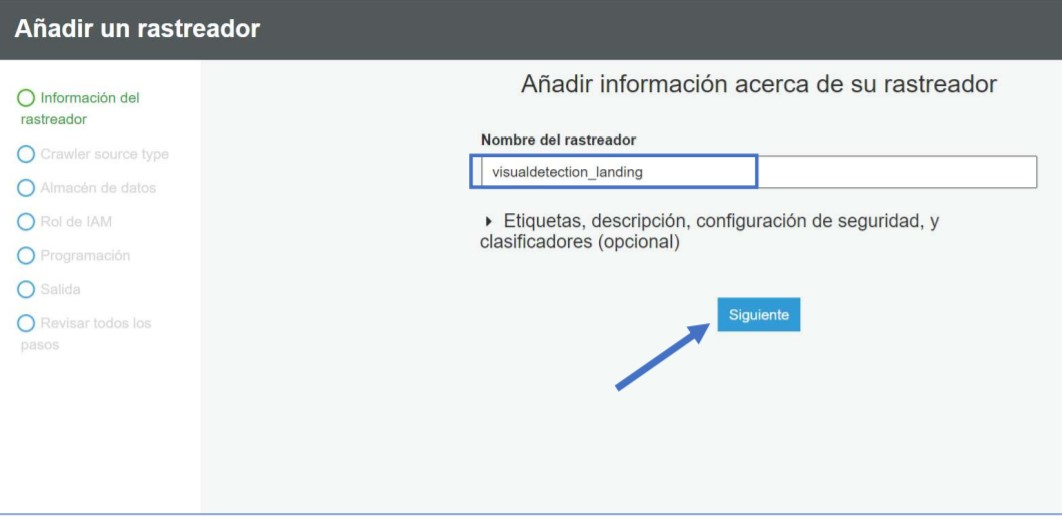
\includegraphics[width=15cm]{./images/3} 
	\end{center}

\newpage
\textbf{1.4.  Seleccionamos la opción : Data Stores (ya que a partir de un csv se creará una tabla)
}

    \begin{center}
		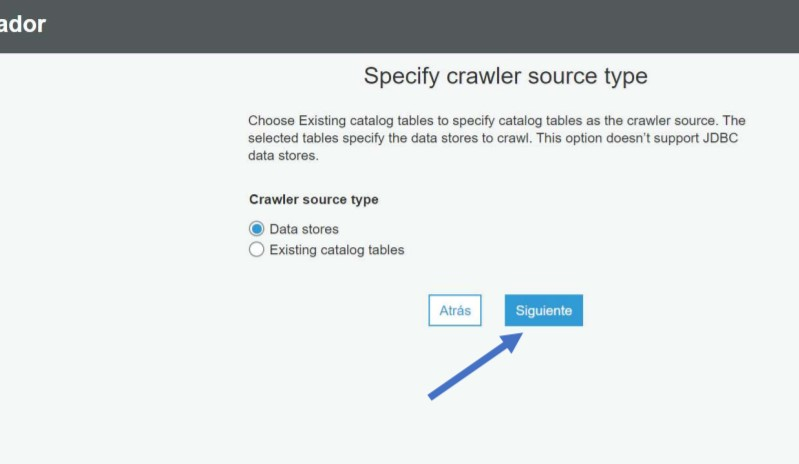
\includegraphics[width=15cm]{./images/4} 
	\end{center}
	
	\newpage
\textbf{1.5.  Elegimos S3, y seleccionamos la carpeta donde se encuentra el archivo csv, clic en Siguiente.
}

    \begin{center}
		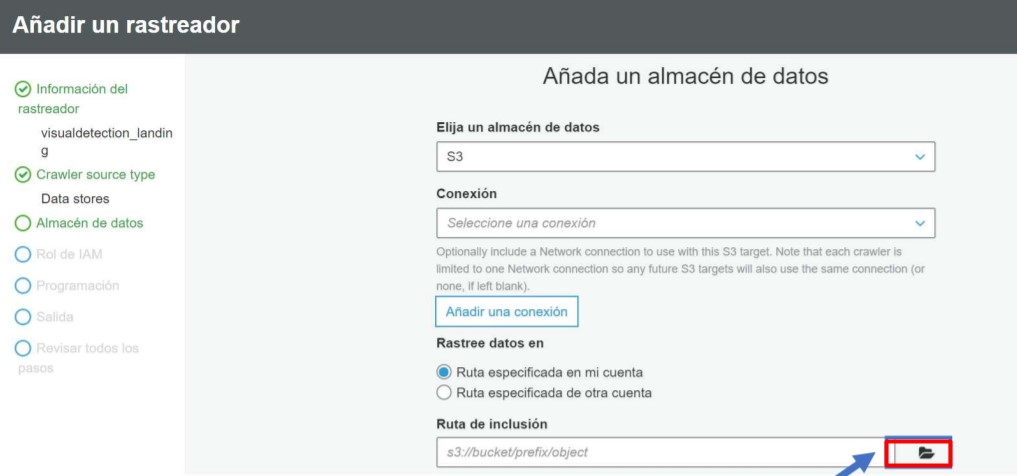
\includegraphics[width=15cm]{./images/5} 
	\end{center}
	
	\newpage
\textbf{1.6.   Seleccionamos hasta la carpeta visualdetecion en S3.
}

    \begin{center}
		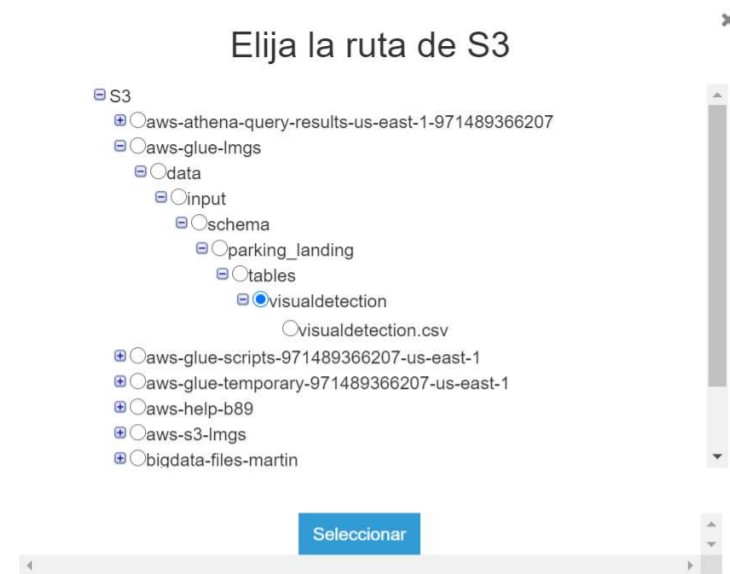
\includegraphics[width=15cm]{./images/6} 
	\end{center}
	
	\newpage
\textbf{1.7. En este caso, solo añadiremos un almacén de datos, elegimos No y clic en Siguiente
}

    \begin{center}
		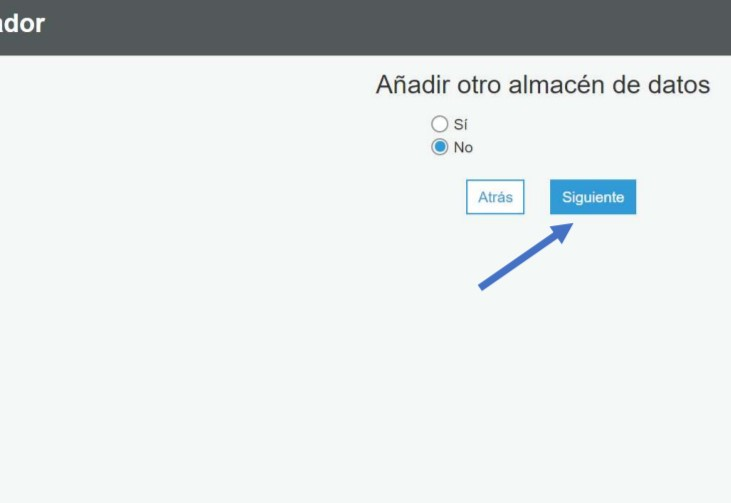
\includegraphics[width=15cm]{./images/7} 
	\end{center}
	
	\newpage
\textbf{1.8.  Creamos un nuevo rol, que tendrá el permiso de leer el archivo csv de S3 y crear una tabla en Glue.
Nombre del rol : AWSGlueServiceRole-Crawler Si ya existe, seleccionar el indicado o concatenarlo con
sus iniciales de sus nombres luego se tiene la opción de definir una periodicidad distinta,de acuerdo a la carga de los datos, si por ejemplo
sé que todos los días a cierta hora, voy a tener un dataset, podría indicar la hora de ejecución automática
de este crawler.
}

    \begin{center}
		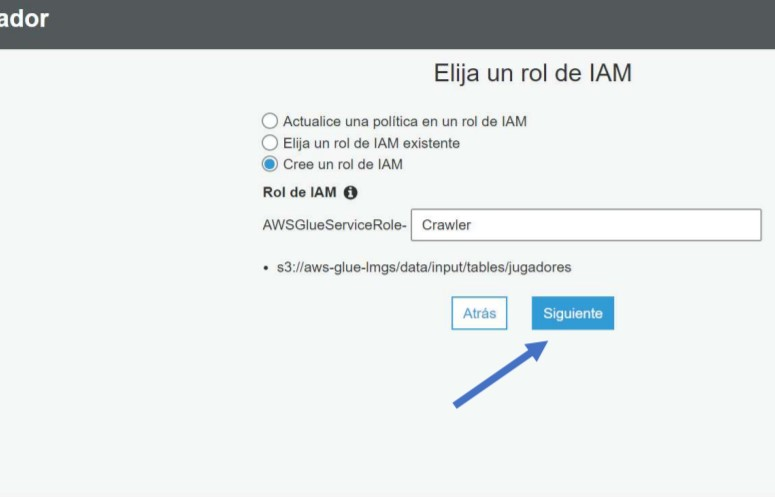
\includegraphics[width=15cm]{./images/8} 
	\end{center}
	
    \begin{center}
		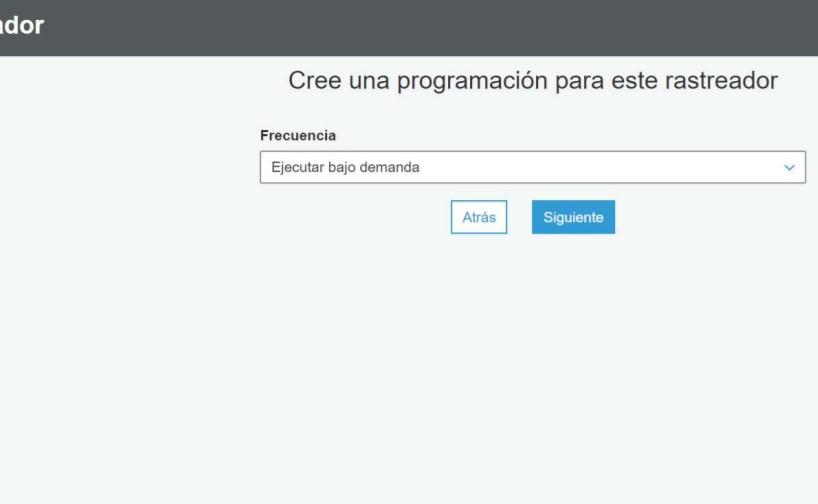
\includegraphics[width=15cm]{./images/9} 
	\end{center}
	
	\newpage
\textbf{1.9.   Añadimos una nueva base de datos, le ponemos como nombre parking landing, clic en Siguiente.
En esta base de datos, se generará de manera automática a partir del dataset que se encuentra en S3,
los datos se leerarán tal cual están en la fuente de donde se descargó todavía no se ha realizado
ninguna transformación.
}

    \begin{center}
		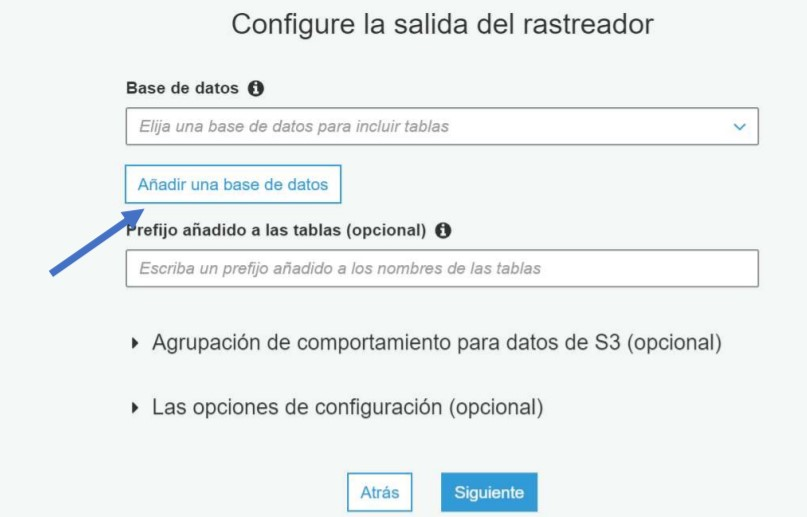
\includegraphics[width=15cm]{./images/10} 
	\end{center}
	
		
	\newpage
\textbf{1.10.  Asignamos el siguiente nombre a la base de datos:
Para no tener inconvenientes, cada uno le pondremos como nombre:
parking landing
}

    \begin{center}
		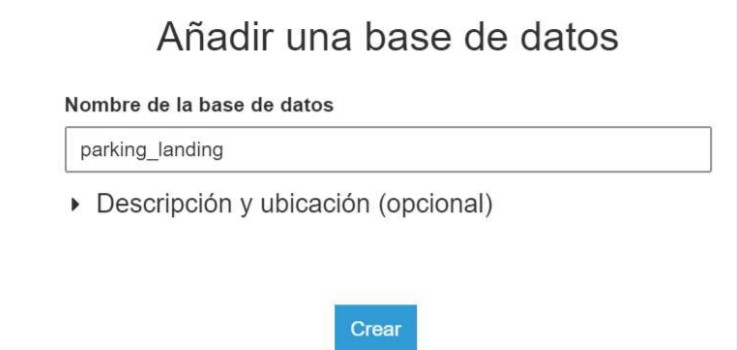
\includegraphics[width=15cm]{./images/11} 
	\end{center}
	
	
		
	\newpage
\textbf{1.11. Le damos clic en Siguiente.
}

    \begin{center}
		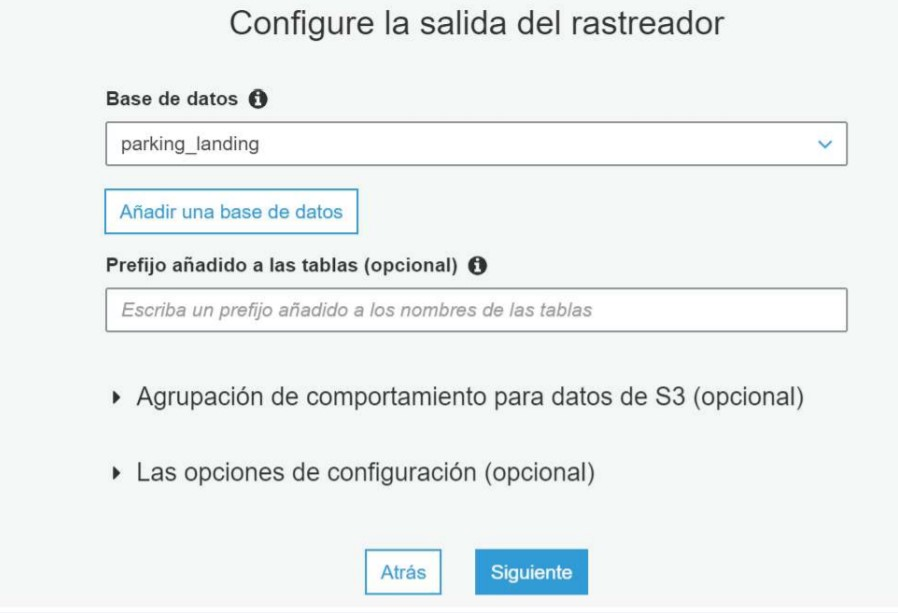
\includegraphics[width=15cm]{./images/12} 
	\end{center}
	
	
	\textbf{1.12.  Clic en Finalizar
}

    \begin{center}
		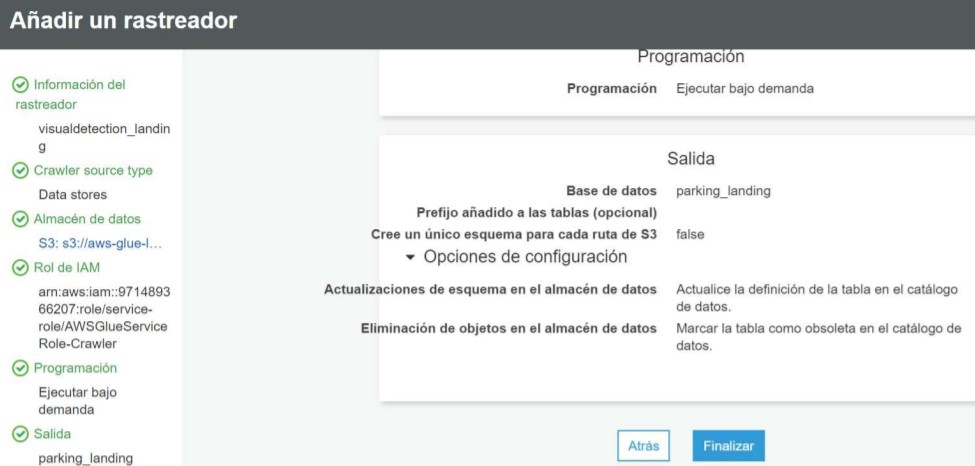
\includegraphics[width=15cm]{./images/13} 
	\end{center}
	
	\textbf{1.13.  Por último para ejecutar este rastreador, le damos clic en ¿Desea ejecutarlo ahora?
}

    \begin{center}
		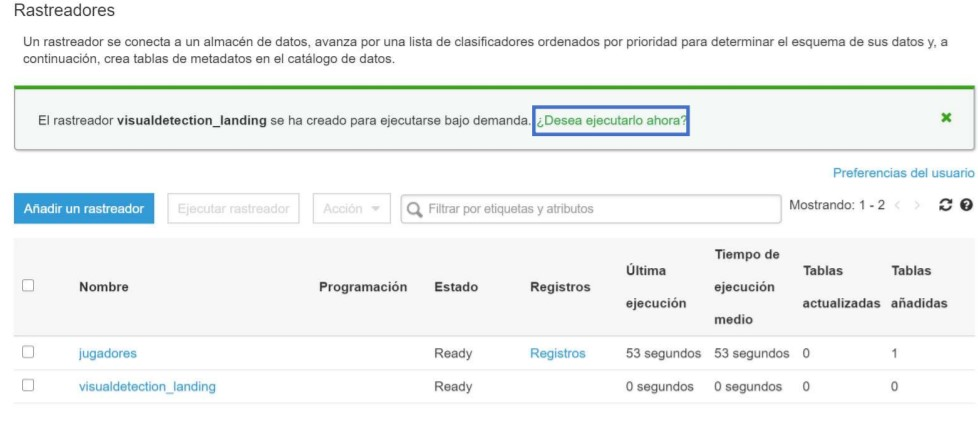
\includegraphics[width=15cm]{./images/14} 
	\end{center}
	
	\textbf{1.14. Después de algunos segundos, el rastreador se detiene y veremos en la última columna que se ha
añadido una nueva tabla en el catálogo de Glue.
}

    \begin{center}
		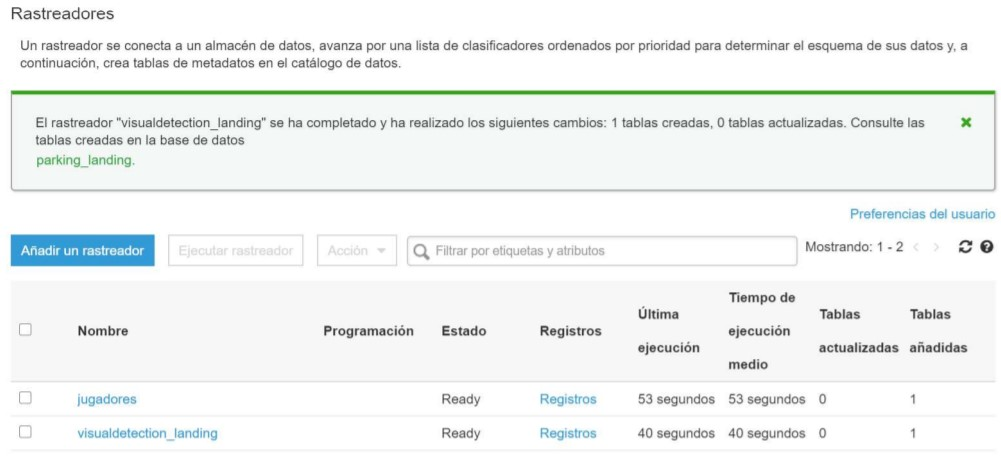
\includegraphics[width=15cm]{./images/15} 
	\end{center}
	
	\textbf{1.15.  Ahora para poder realizar una consulta SQL en el servicio de Athena, entramos al servicio.
}

    \begin{center}
		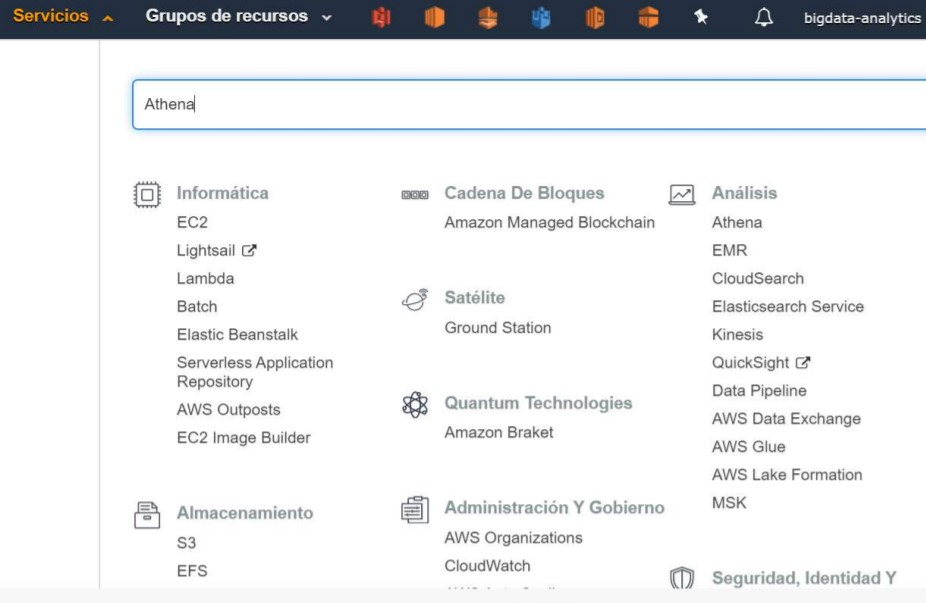
\includegraphics[width=15cm]{./images/16} 
	\end{center}
	
	\textbf{1.16.  Antes de realizar una consulta SQL en Athena, debemos realizar la siguiente configuración.
Clic en Settings.
}

    \begin{center}
		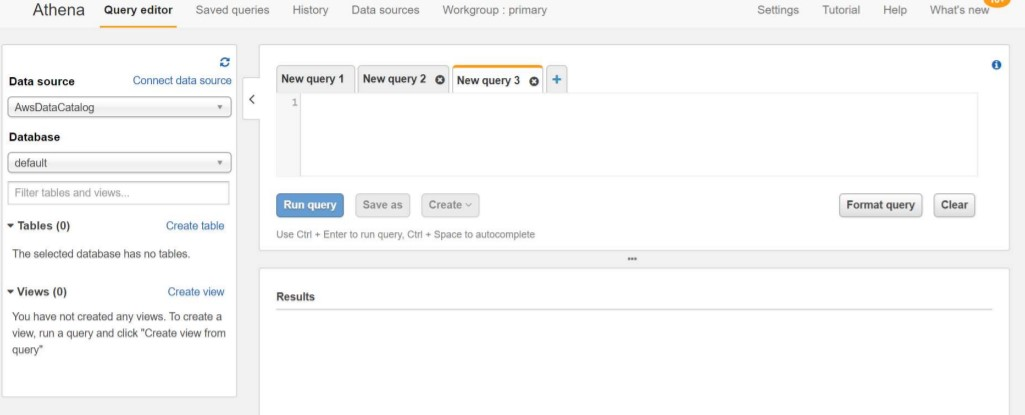
\includegraphics[width=15cm]{./images/17} 
	\end{center}
	
	
		\textbf{1.17.  Indicamos el bucket que hemos creado, y le agregamos /data/output/, en esta ruta se guardarán 2
archivos (1 el resultado de los querys y el segundo con la metadata).
}

    \begin{center}
		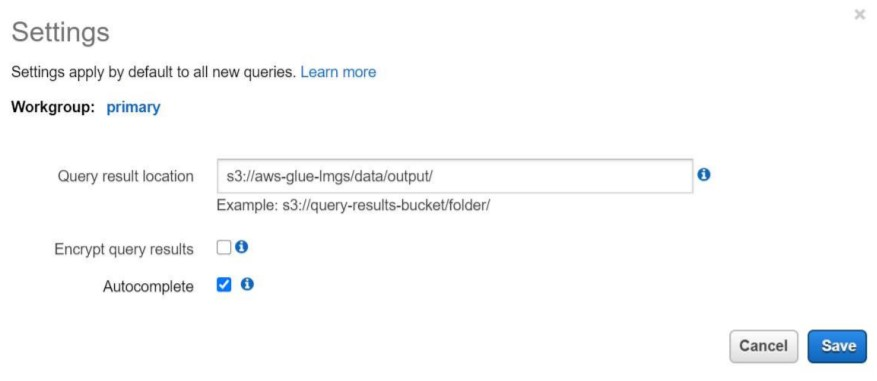
\includegraphics[width=15cm]{./images/18} 
	\end{center}
	
	
	
		\textbf{1.18. Ahora podremos ejecutar consultas SQL en Athena. 
Clic en Settings.
}

    \begin{center}
		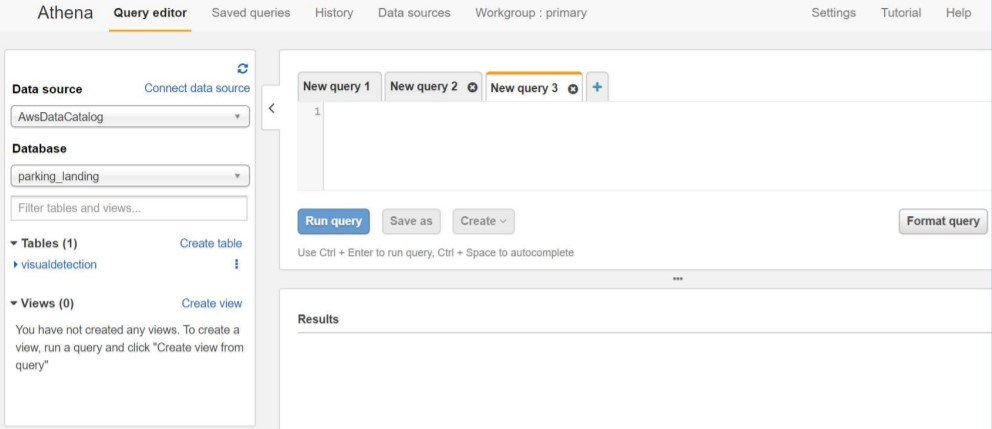
\includegraphics[width=15cm]{./images/19} 
	\end{center}
	
	
		\textbf{1.19.  AEjecutamos algunos querys para probar Athena:
SELECT * FROM parking landing.visualdetection limit 10;
SELECT * FROM parking landing.visualdetection where camera = 'A';
Clic en Settings.
}

    \begin{center}
		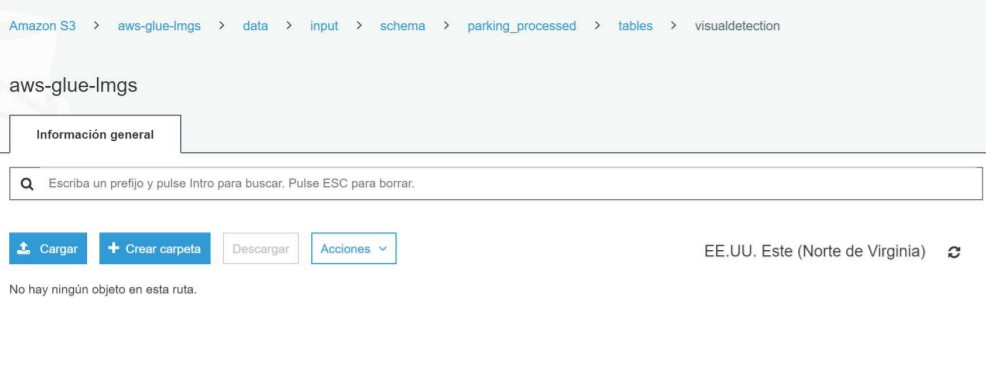
\includegraphics[width=15cm]{./images/20} 
	\end{center}
	
	
		\textbf{1.20.  Luego, nos vamos a Glue para crear el job de transformación
Clic en Settings.
}

    \begin{center}
		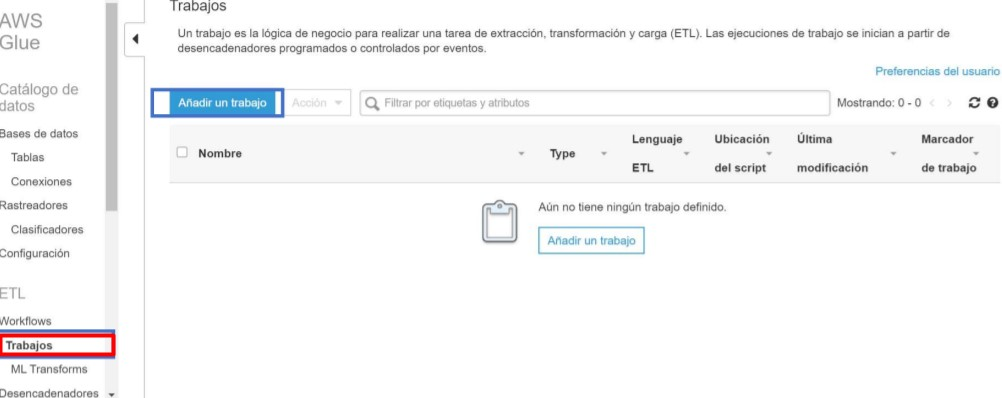
\includegraphics[width=15cm]{./images/21} 
	\end{center}
	
	
		\textbf{1.21. Definir como nombre del job : visualdetecion processed, clic en siguiente.
Clic en Settings.
}

    \begin{center}
		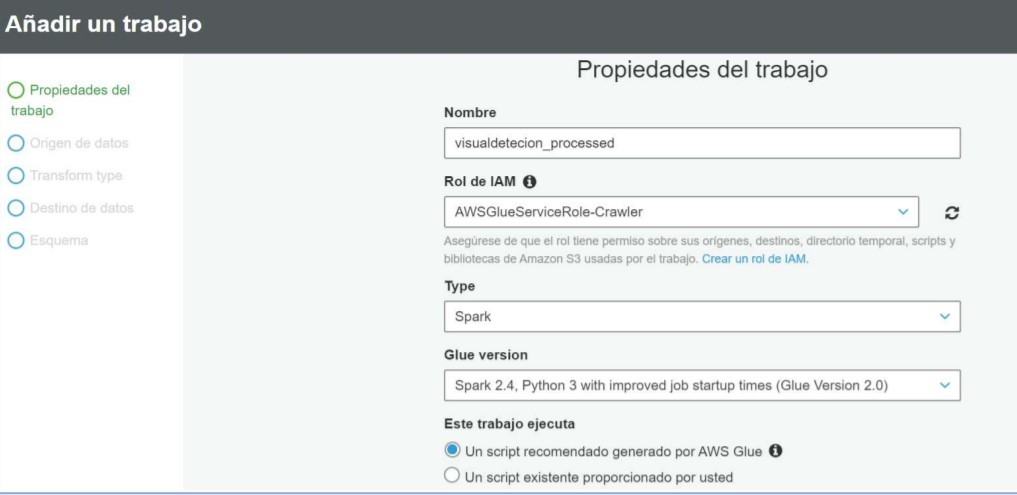
\includegraphics[width=15cm]{./images/22} 
	\end{center}
	
	
		\textbf{1.22.  Seleccionamos la tabla visualdetection que está dentro de la base de datos que hemos creado cada uno
(es la que se encuentra en formato csv), clic en Siguiente.
Clic en Settings.
}

    \begin{center}
		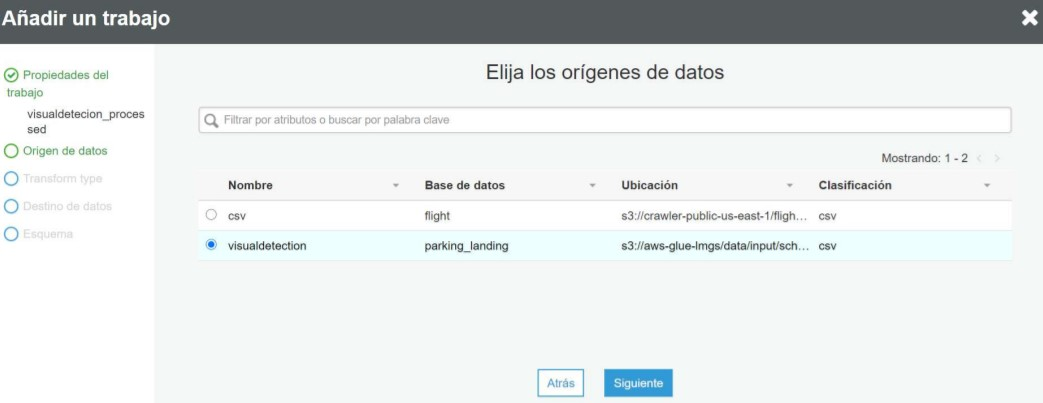
\includegraphics[width=15cm]{./images/23} 
	\end{center}
	
	
		\textbf{1.23.  Elegimos cambiar esquema y siguiente.
Clic en Settings.
}

    \begin{center}
		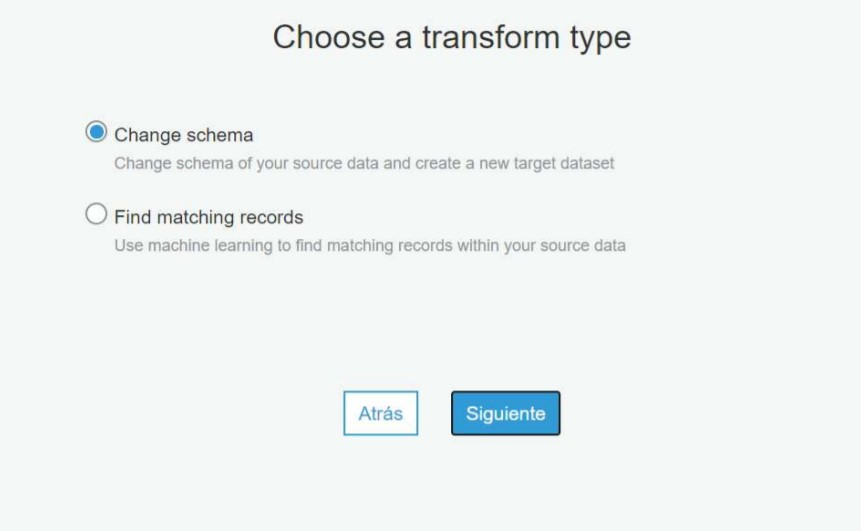
\includegraphics[width=15cm]{./images/24} 
	\end{center}
	
	
		\textbf{1.24. Modificar el nombre de bucket por el nuestro.
}

    \begin{center}
		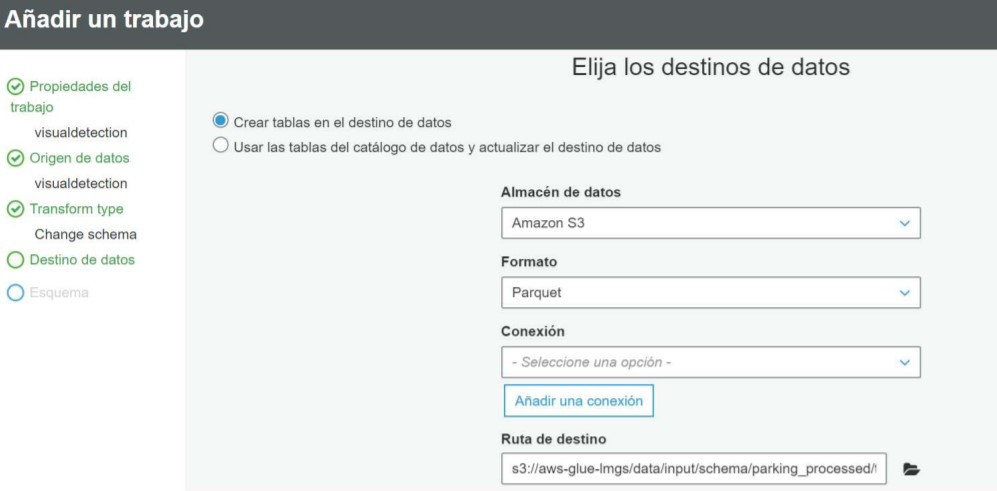
\includegraphics[width=15cm]{./images/25} 
	\end{center}
	
	
\end{document}